\documentclass[aspectratio=169, 12pt]{beamer}    %set the aspect ratio to 16:9
%5\documentclass[]{beamer}  %set the aspect ratio to 4:3
\usepackage[dct]{../../inst/rmarkdown/templates/autbeamer/skeleton/AUTtheme}     % AUT theme                                  

% title page content
\title[Beamer title]
{This is the main (long or short) title. This is the main (long or short) title.
%This is the main (long or short) title
}
%\subtitle{This is a (long or short) subtitle}
\author[Sarah, Wenqiang]{Sarah Marshall\inst{1}, Wenqiang Liu\inst{2}}
\institute
{\inst{1}  Engineering, Computer Mathematical Sciences (ECMS) \\
\inst{2}  Engineering, Computer Mathematical Sciences (ECMS) \\
\inst{3}  Engineering, Computer Mathematical Sciences (ECMS) 
}
\date{The Name of the Conference \\ The Name of the Venue \\
7 February 2023
}


\bibliographystyle{ieeetr}

% \titlegraphic{\includegraphics[width=\paperwidth, height = \paperheight]{images/Title_bg_image.png}}
%\titlegraphic{titlegraphic}

\begin{document}
% \begin{titleframe}
%     \maketitle
% \end{titleframe}

\begin{frame}
    \maketitle
\end{frame}


\begin{sectionframe}
\frametitle{Table of Contents}
\tableofcontents[hideallsubsections]
\end{sectionframe}



\section{Frames}


\subsection{Frame Sizes}
\begin{frame}[fragile = singleslide]{Frame Sizes}

The template can be used to create $16\times9$ or $4 \times 3$ slides.
The resolution of the background images get updated automatically.

\begin{itemize}
\item To create $16 \times 9$ slides
\begin{verbatim}
\documentclass[aspectratio=169]{beamer} 
\end{verbatim}

\item To create $4 \times 3$ slides
\begin{verbatim}
\documentclass[]{beamer}  
\end{verbatim}

\end{itemize} 


\end{frame}

\subsection{Loading the AUTTheme}
\begin{frame}[fragile = singleslide]{Loading the AUTTheme}
 
\begin{verbatim}
\usepackage{AUTtheme}  
\end{verbatim}

The DCT colour theme is the default, however it can be forced as follows:
\begin{verbatim}
\usepackage[dct]{AUTtheme}  
\end{verbatim}


\end{frame}

\subsection{Compiling with AUTTheme}
\begin{frame}[fragile = singleslide]{Compiling with AUTTheme}
 
\verb|lualatex| is recommended.

\end{frame}



\subsection{Frame Types}
\begin{frame}[fragile = singleslide]{Frame Types}

This template uses three types of frames
\begin{itemize}
 \item \alert{Title page:}
 \begin{verbatim}
\begin{frame}
  \maketitle 
\end{frame}
\end{verbatim}
 
 \item \alert{Section frame:}
 \begin{verbatim}
\begin{sectionframe}\frametitle{Frame Title}
 Content for right hand side of slide
\end{sectionframe}
\end{verbatim}

\item \alert{Default frame:}
\begin{verbatim}
\begin{frame}{Frame Title}
Frame content
\end{frame}
\end{verbatim}

\end{itemize}
\end{frame}


% \begin{frame}[fragile]{How to create title page}
%   A title page can be created the traditional way, using the "maketitle" or "titlepage" commands in a frame environment.

% \begin{columns}
%     \column{0.6\textwidth}
%     \begin{alertblock}{Method two}
%     \begin{verbatim}
%     \begin{titleframe}
%         \maketitle
%     \end{titleframe}
%     \end{verbatim}
%     \end{alertblock}
%     \column{0.4\textwidth}
%         You can build a title page based on this code in the box on the left side.
% \end{columns}
% \end{frame}

\subsection{New sectionframe environment}
\begin{frame}[fragile]{Create contents page using sectionframe environment}
\begin{columns}
\column{0.6\textwidth}
\begin{alertblock}{Example Code}

\begin{verbatim}
\begin{sectionframe}
\frametitle{Table of Contents}
\tableofcontents[
     hideallsubsections]
\end{sectionframe}
\end{verbatim}

\end{alertblock}

\column{0.4\textwidth}
 You can use \verb|\tableofcontents| or build your own table of contents page.
\end{columns}
\end{frame}


\begin{frame}[fragile]{Slides at beginning of section}

By default two \verb|sectionpage| is displayed at the start of each section.
The first contains the section name and the second contains 
 a table of contents.

Both can be edited within the \verb|.tex| file.

e.g. To switch off use within the \verb|.tex| file.
\begin{verbatim}
\AtBeginSection{}
\end{verbatim}



\end{frame}

\section{Slide Content}



\subsection{Bulleted lists}
\begin{frame}{List}
    \begin{itemize}
        \item Item 1
        \begin{itemize}
            \item Subitem 1.1
            \begin{itemize}
                \item Subsubitem  1.1.1
                \item Subsubitem 1.1.2
            \end{itemize}
%            \item Text visible on slide 1.2
%            \begin{itemize}
%                \item Text visible on slide 1.2.1
%                \item Text visible on slide 1.2.2
%            \end{itemize}
        \end{itemize}
        \item Item 2 
        \item Item 3
        % \item Text visible on slide 4
        % \item Text visible on slide 5
    \end{itemize}
\end{frame}



\begin{sectionframe}
    \frametitle{Example: create a one-off table of contents}
    \setlength{\parskip}{0ex}
\tableofcontents[ 
    	currentsubsection, 
        sectionstyle=show/shaded, 
        subsectionstyle=show/show/hide,
    ] 
    

 
\end{sectionframe}

\subsection{Ordered Lists}
\begin{frame}{Ordered Lists}
    \begin{enumerate}%[default]
    \item Point 1 
    \item Point 2 
    \begin{enumerate}[a.]
        \item part a 
            \begin{enumerate}[i.]
                \item another point
                \item another point
            \end{enumerate}
        \item part 2 
            \begin{itemize}%[i]
                \item another point
                \item another point
            \end{itemize}
    \end{enumerate}
    \item Point 3 
    \item Point 4 
    \end{enumerate}
\end{frame}



\subsection{Highlights and Colours}
\begin{frame}[fragile]{Highlights and Colours}

\begin{itemize}
\item 
    \colorbox{orange}{Highlight with colorbox} \\
    
\item 
    We do not only have "colorbox" method, but we also \textbf{have other highlight methods}. \alert{For example}, some \textcolor{green}{important text} will be \textcolor{blue}{highlighted here.} \\
    
\item     
    The AUT-themed orange text can be obtained using \verb|\alert{text}| or \verb|\textcolor{deeporangeAUT}{text}|.
\end{itemize}
    
    
\end{frame}

\subsection{Blocks}
\begin{frame}{Alert block with deep orange}
        %  alert block
    \begin{alertblock}{Alert block}
        This is the orange block, we also could use other colors for blocks.
    \end{alertblock}
    
    \begin{alertblock}{Alert block}
        Gosh, what should I do!!!
    \end{alertblock}  
\end{frame}


\subsection{Columns}
\begin{frame}{Columns}
     % Get the performance of column
    \begin{columns}
    \column{0.5\textwidth}
    This is a text in the first column.
    $$E = mc^2 $$
    \begin{itemize}
        \item The first term
        \item The second term
    \end{itemize}
    
    \column{0.5\textwidth}
    This is a text in the second column.
    \end{columns}
\end{frame}

% in three columns
\begin{frame}{Three columns}
    \begin{columns}
        \column{0.3\textwidth}
        This is the first column content.
        \column{0.3\textwidth}
        This is the second column content.
        \column{0.3\textwidth}
        This is the third column content.
    \end{columns}
\end{frame}


\subsection{Citations}
\begin{frame}{Literature review}
    You can site a paper like this \cite{teichmann2019machine, buehler2019deep}
\end{frame}

\section{Maths and Floats}
\subsection{Mathematical formula}
\begin{frame}{Using math formula}
In this slide, we insert an equation(\ref{E1}), which is the definition of $y$.
\begin{equation}
    \label{E1}
    y = 
    \begin{cases}
    \frac{1}{f(x)},\ f(x) \neq 0 \\
    f(x), \ f(x) = 0
    \end{cases}
\end{equation}
\end{frame}


\subsection{Tables}
\begin{frame}
\frametitle{Insert a table}
This results are shown in Table \ref{T1}
\begin{table}[ht]   
    \caption{A sample table}
    \label{T1}
    \centering
    \begin{tabular}{p{1.5cm}|p{1.5cm}|p{1.5cm}}
    \hline
    Metrics     &   M1      &   M2      \\
    \hline
    Accuracy    &   84\%    &   88\%     \\
    Precision   &   91\%    &   90\%     \\
    Recall      &   75\%    &   77\%     \\
    \hline
    \end{tabular}
\end{table}
\end{frame}

\subsection{Figures}
\begin{frame}{Insert a sample figure}
The data-set information is shown in Figure \ref{dataset}.
\begin{figure}
    \centering
    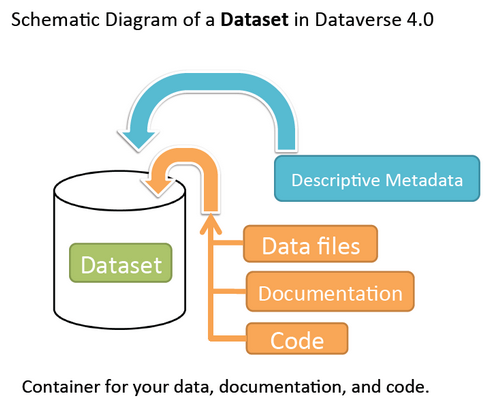
\includegraphics[width=6cm,height=4.5cm]{figs/dataset.png}
    \caption{A sample picture}
    \label{dataset}
\end{figure}
\end{frame}

\section{References}

\begin{frame}{References}
% Show the references
\bibliography{literature}
\end{frame}

\begin{sectionframe}

\begin{center}
{\Huge
\alert{
Thank you very much for your attention!
}
}
\end{center}
\end{sectionframe}


\begin{titleframe}
\begin{center}
{
\huge

\vspace{1cm}

\textcolor{white}{
The end
}
\vspace{1cm}

}
\end{center}
\end{titleframe}

\begin{titleframe}
\end{titleframe}


\end{document}
\appendix
\section{Appendix}
\begin{sectionframe}
    \frametitle{Appendix}
\end{sectionframe}

\section{Animations}

\subsection{Ordered bulleted list}
\begin{frame}{List item with animation}
    \begin{itemize}
        \item<1-> Text visible on slide 1
        \begin{itemize}
            \item<2-> Text visible on slide 1.1
            \begin{itemize}
                \item<3-> Text visible on slide 1.1.1
                \item<4-> Text visible on slide 1.1.2
            \end{itemize}
            \item<5-> Text visible on slide 1.2
            \begin{itemize}
                \item<6-> Text visible on slide 1.2.1
                \item<7-> Text visible on slide 1.2.2
            \end{itemize}
        \end{itemize}
        \item<8-> Text visible on slide 2 
        \item<9-> Text visible on slide 3
        % \item<10-> Text visible on slide 4
        % \item<11-> Text visible on slide 5
    \end{itemize}
\end{frame}

\subsection{Pause function}
\begin{frame}{The animation function via "pause"}
    In this slide \pause
    the text will be partially visible \pause
    And friendly everything will be there    
\end{frame}


% \begin{frame}{Section page}
    
% \end{frame}

% \begin{frame}{Outline}
    
% \end{frame}

% \begin{frame}{Table of Contents}
    
% \end{frame}

% \begin{frame}{Contents}
    
% \end{frame}

\end{document}